\documentclass[12pt]{article}
\usepackage{amsmath, amsthm, amssymb}
\usepackage{hyperref}
\usepackage{verbatim}
\usepackage[top=1.0in, bottom=1.0in, left=1.0in, right=1.0in]{geometry}
\usepackage{color}
\pagestyle{plain}

\usepackage{sectsty}
\allsectionsfont{\sffamily}

\usepackage{tkz-graph}
\usetikzlibrary{arrows}
\usetikzlibrary{shapes}
\usepackage[position=bottom]{subfig}

\makeatletter
\newtheorem*{rep@theorem}{\rep@title}
\newcommand{\newreptheorem}[2]{
\newenvironment{rep#1}[1]{
 \def\rep@title{#2 \ref{##1}}
 \begin{rep@theorem}}
 {\end{rep@theorem}}}
\makeatother

\theoremstyle{plain}
\newtheorem{thm}{Theorem}[section]
\newreptheorem{thm}{Theorem}
\newtheorem{prop}[thm]{Proposition}
\newreptheorem{prop}{Proposition}
\newtheorem{lem}[thm]{Lemma}
\newreptheorem{lem}{Lemma}
\newtheorem{conjecture}[thm]{Conjecture}
\newreptheorem{conjecture}{Conjecture}
\newtheorem{cor}[thm]{Corollary}
\newreptheorem{cor}{Corollary}
\newtheorem{prob}[thm]{Problem}

\newtheorem*{KernelLemma}{Kernel Lemma}
\newtheorem*{BK}{Borodin-Kostochka Conjecture}
\newtheorem*{BK2}{Borodin-Kostochka Conjecture (restated)}
\newtheorem*{Reed}{Reed's Conjecture}
\newtheorem*{ClassificationOfd0}{Classification of $d_0$-choosable graphs}


\theoremstyle{definition}
\newtheorem{defn}{Definition}
\theoremstyle{remark}
\newtheorem*{remark}{Remark}
\newtheorem*{problem}{Problem}
\newtheorem{example}{Example}
\newtheorem*{question}{Question}
\newtheorem*{observation}{Observation}

\newcommand{\fancy}[1]{\mathcal{#1}}
\newcommand{\C}[1]{\fancy{C}_{#1}}


\newcommand{\IN}{\mathbb{N}}
\newcommand{\IR}{\mathbb{R}}
\newcommand{\G}{\fancy{G}}
\newcommand{\CC}{\fancy{C}}
\newcommand{\D}{\fancy{D}}
\newcommand{\T}{\fancy{T}}
\newcommand{\B}{\fancy{B}}
\renewcommand{\L}{\fancy{L}}
\newcommand{\HH}{\fancy{H}}

\newcommand{\inj}{\hookrightarrow}
\newcommand{\surj}{\twoheadrightarrow}

\newcommand{\set}[1]{\left\{ #1 \right\}}
\newcommand{\setb}[3]{\left\{ #1 \in #2 : #3 \right\}}
\newcommand{\setbs}[2]{\left\{ #1 : #2 \right\}}
\newcommand{\card}[1]{\left|#1\right|}
\newcommand{\size}[1]{\left\Vert#1\right\Vert}
\newcommand{\ceil}[1]{\left\lceil#1\right\rceil}
\newcommand{\floor}[1]{\left\lfloor#1\right\rfloor}
\newcommand{\func}[3]{#1\colon #2 \rightarrow #3}
\newcommand{\funcinj}[3]{#1\colon #2 \inj #3}
\newcommand{\funcsurj}[3]{#1\colon #2 \surj #3}
\newcommand{\irange}[1]{\left[#1\right]}
\newcommand{\join}[2]{#1 \mbox{\hspace{2 pt}$\ast$\hspace{2 pt}} #2}
\newcommand{\djunion}[2]{#1 \mbox{\hspace{2 pt}$+$\hspace{2 pt}} #2}
\newcommand{\parens}[1]{\left( #1 \right)}
\newcommand{\brackets}[1]{\left[ #1 \right]}
\newcommand{\DefinedAs}{\mathrel{\mathop:}=}

\newcommand{\mic}{\operatorname{mic}}
\newcommand{\AT}{\operatorname{AT}}
\newcommand{\col}{\operatorname{col}}
\newcommand{\ch}{\operatorname{ch}}
\newcommand{\type}{\operatorname{type}}
\newcommand{\nonsep}{\bar{S}}

\def\adj{\leftrightarrow}
\def\nonadj{\not\!\leftrightarrow}

\newcommand\restr[2]{{% we make the whole thing an ordinary symbol
  \left.\kern-\nulldelimiterspace % automatically resize the bar with \right
  #1 % the function
  \vphantom{\big|} % pretend it's a little taller at normal size
  \right|_{#2} % this is the delimiter
  }}

\def\D{\fancy{D}}
\def\C{\fancy{C}}
\def\A{\fancy{A}}

\newcommand{\case}[2]{{\bf Case #1.}~{\it #2}~~}

\title{Edge Lower Bounds for List Critical Graphs, via Discharging}
\author{Dan and Landon}

\begin{document}
\maketitle

\section{Introduction}
%For a graph $G$, let $d(G)$ be the average degree of $G$. 
%A \emph{Gallai tree} is a connected graph in which each block is a clique or an odd cycle.
%Let $\T_k$ be the collection of Gallai trees with maximum degree at most $k-1$, excluding $K_k$. 

A \emph{proper coloring} of a graph $G$ assigns colors to vertices so that adjacent vertices receive distinct colors.  A graph $G$ is \emph{$k$-colorable} if $G$ has a proper coloring using at most $k$ colors.
The \emph{chromatic number} $\chi(G)$ of $G$ is the least $k$ for which $G$ is $k$-colorable. A graph $G$ is \emph{$k$-chromatic} when $\chi(G) = k$, and $G$ is \emph{$k$-critical} when $G$ is not $(k-1)$-colorable, but every proper subgraph of $G$ is $(k-1)$-colorable.  Every $k$-critical graph $G$ is $k$-chromatic since, for any vertex $v$, we can extend a $(k-1)$-coloring of $G-v$ to a $k$-coloring of $G$, by giving $v$ a new color.  If $G$ is $k$-chromatic, then any minimal $k$-chromatic subgraph of $G$ is $k$-critical.  As a result, many questions about $k$-chromatic graphs reduce to questions about $k$-critical graphs, which have more structure.  Dirac \cite{dirac1951note} introduced critical graphs in 1951.  Since every $k$-critical graph $G$ has minimum degree at least $k-1$, clearly $2\size{G} \ge (k-1)\card{G}$.  Much work has focused on determining the minimum number of edges in a $k$-critical graph. In 1957, Dirac \cite{dirac1957theorem} generalized Brooks' theorem \cite{brooks1941colouring} by showing that any $k$-critical graph $G$ with $k \ge 4$ and $\card{G} \ge k+2$ must satisfy 

\[2\size{G} \ge (k-1)\card{G} + k-3.\]

In 1963, Gallai \cite{gallai1963kritische} strengthened this bound for large $\card{G}$.  Let 
\[g_k(n, c) \DefinedAs \parens{k-1 + \frac{k-3}{(k-c)(k-1) + k-3}}n.\]
Gallai showed that every $k$-critical graph $G$ with $k \ge 4$ and $\card{G} \ge k+2$ satisfies $2\size{G} \ge g_k(\card{G}, 0)$.  In 1997, Krivelevich \cite{krivelevich1997minimal} strengthened this lower bound to $g_k(\card{G}, 2)$.  In 2003, Kostochka and Stiebitz \cite{kostochkastiebitzedgesincriticalgraph} further strengthened this bound, for $k \ge 6$, to $2\size{G} \ge g_k(\card{G}, (k-5)\alpha_k)$, where

\[\alpha_k \DefinedAs \frac12 - \frac{1}{(k-1)(k-2)}.\]

Table \ref{tab:1} gives the values of these bounds for small $k$.  In 2012, Kostochka and Yancey \cite{kostochkayancey2012ore} had a remarkable breakthrough on this problem, showing that every $k$-critical graph $G$ with $k \ge 4$ must satisfy

\[\size{G} \ge \ceil{\frac{(k+1)(k-2)\card{G} - k(k-3)}{2(k-1)}}.\]
Moreover, their bound is tight for $k=4$ and $n \ge 6$ as well as for infinitely many values of $\card{G}$ for each $k \ge 5$.  This bound has numerous applications to coloring problems, including a short proof of Gr\"otsch's theorem that triangle-free planar graphs are $3$-colorable \cite{kostochka2012oregrotsch} and short proofs of the results on coloring with respect to Ore degree in \cite{kierstead2009ore, rabern2010a, krs_one}. 

Given these applications to coloring problems, it is natural to study the same problem for more general types of coloring.  In this article, we prove better lower bounds on the number of edges in a critical graph, for both the list coloring and online list coloring problems.  To state our results we need some definitions.

\emph{List coloring} was introduced by Vizing \cite{vizing1976} and independently by Erd\H{o}s, Rubin, and Taylor \cite{erdos1979choosability}.  Let $G$ be a graph. A list assignment on $G$ is a function $L$ from $V(G)$ to the subsets of $\IN$.   A graph $G$ is \emph{$L$-colorable} if $G$ has a proper coloring $\pi$ such that $\pi(v)\in L(v)$ for all $v$.   A graph $G$ is \emph{$L$-critical} if $G$ is not $L$-colorable, but every proper subgraph $H$ of $G$ is $\restr{L}{V(H)}$-colorable. For $\func{f}{V(G)}{\IN}$, a list assignment $L$ is an \emph{$f$-assignment} if $\card{L(v)} = f(v)$ for each $v \in V(G)$.  If $f(v) = k$ for all $v \in V(G)$, then we also call an $f$-assignment a $k$-assignment.  We say that $G$ is \emph{$f$-choosable} if $G$ is $L$-colorable for every $f$-assignment $L$.  
We say that $G$ is $k$-list-critical if $G$ is $L$-critical for some $k$-list assignment $L$. %HK
The best, known-lower bound on the number of edges in a $k$-list-critical graph, was given by Kostochka and Stiebitz \cite{kostochkastiebitzedgesincriticalgraph} in 2003. %HK edits
It states that for $k \ge 9$ and every graph $G \ne K_k$ if $G$ is a $k$-list-critical graph, then $2\size{G} \ge g_k(\card{G}, \frac13 (k-4)\alpha_k)$.  We improve their bound to $2\size{G} \ge g_k(\card{G}, (k-3)\alpha_k)$ for $k\ge7$ (see Table \ref{tab:1}).

\emph{Online list coloring} was independently introduced by Zhu \cite{zhu2009online} and Schauz \cite{schauz2009mr} (Schauz called it \emph{paintability}). Let $G$ be a graph and $\func{f}{V(G)}{\IN}$.  We say that $G$ is \emph{online $f$-choosable} if $f(v) \ge 1$ for all $v \in V(G)$ and for every $S \subseteq V(G)$ there is an independent set $I \subseteq S$ such that $G-I$ is online $f'$-choosable where $f'(v) \DefinedAs f(v)$ for $v \in V(G) - S$ and $f'(v) \DefinedAs f(v) - 1$ for $v \in S - I$.
Observe that if a graph is online $f$-choosable then it is $f$-choosable. 
When $f(v) \DefinedAs k-1$ for all $v \in V(G)$, we say that $G$ is \emph{online $k$-list-critical} if $G$ is not online $f$-choosable, 
but every proper subgraph $H$ of $G$ is online $\restr{f}{V(H)}$-choosable.  In 2012, Riasat and Schauz \cite{riasat2012critically} showed that Gallai's bound  $2\size{G} \ge g_k(\card{G}, 0)$ holds for online $k$-list-critical graphs.  We improve this for $k \ge 7$ by proving the same bound as we have for list coloring: $2\size{G} \ge g_k(\card{G}, (k-3)\alpha_k)$.

%Our main theorem shows that a graph either has many edges or an induced subgraph which has a certain kind of good orientation.  To describe these good orientations we need a few definitions. A subgraph $H$ of a directed multigraph $D$ is called \emph{Eulerian} if $d^-_H(v) = d^+_H(v)$ for every $v \in V(H)$.  We call $H$ \emph{even} if $\size{H}$ is even and \emph{odd} otherwise.  Let $EE(D)$ be the number of even, spanning, Eulerian subgraphs of $D$ and $EO(D)$ the number of odd, spanning, Eulerian subgraphs of $D$.  Note that the edgeless subgraph of $D$ is even and hence we always have $EE(D) > 0$.

%Let $G$ be a graph and $\func{f}{V(G)}{\IN}$.  We say that $G$ is \emph{$f$-Alon-Tarsi} (for brevity, \emph{$f$-AT}) if $G$ has an orientation $D$ where $f(v) \ge d_{D}^+(v) + 1$ for all $v \in V(D)$ and $EE(D) \ne EO(D)$. One simple way to achieve $EE(D) \ne EO(D)$ is to have $D$ be acyclic since then we have $EE(D) = 1$ and $EO(D) = 0$.  In this case, ordering the vertices so that all edges point the same direction and coloring greedily shows that $G$ is $f$-choosable. If we require $f$ to be constant, we get the familiar \emph{coloring number} $\col(G)$; that is, $\col(G)$ is the smallest $k$ for which $G$ has an acyclic orientation $D$ with $k \ge d_{D}^+(v) + 1$ for all $v \in V(D)$.  Alon and Tarsi \cite{Alon1992125} generalized from the acyclic case to arbitrary $f$-AT orientations.

%\begin{lem}\label{AlonTarsi}
%	If a graph $G$ is $f$-AT for $\func{f}{V(G)}{\IN}$, then $G$ is $f$-choosable.
%\end{lem}

%\noindent Schauz \cite{schauz2010flexible} extended this result to online $f$-choosability.

%\begin{lem}\label{Schauz}
%	If a graph $G$ is $f$-AT for $\func{f}{V(G)}{\IN}$, then $G$ is online $f$-choosable.
%\end{lem}

For a graph $G$, we define $\func{d_0}{V(G)}{\IN}$ by $d_0(v) \DefinedAs d_G(v)$.  The $d_0$-choosable graphs were first characterized by Borodin \cite{borodin1977criterion} and independently by Erd\H{o}s, Rubin and Taylor \cite{erdos1979choosability}.  The connected graphs which are not $d_0$-choosable are precisely the Gallai trees (connected graphs in which every block is complete or an odd cycle). The generalization to a characterization of $d_0$-AT graphs was first given in \cite{Hladky} by Hladk{\`y}, Kr{\'a}l and Schauz. 

%We prove the following general theorem saying that either a graph has many edges or has an induced $f_H$-AT subgraph $H$ where %$f_H$ basically gives the number of colors we would expect the vertices to have left in their lists after $\delta(G)$-coloring %$G-H$.

%\begin{defn}
%	A graph $G$ is \emph{AT-reducible} to $H$ if $H$ is a nonempty induced subgraph of $G$ which is $f_H$-AT where $f_H(v) %\DefinedAs \delta(G) + d_H(v) - d_G(v)$ for all $v \in V(H)$.  
%	If $G$ is not AT-reducible to any nonempty induced subgraph, then it is \emph{AT-irreducible}.
%\end{defn}

%\begin{repthm}{EdgeBoundEuler}
%	If $G$ is an AT-irreducible graph with $\delta(G) \ge 4$ and $\omega(G) \le \delta(G)$, then $2\size{G} \ge %g_{\delta(G)+1}(\card{G}, c)$ where $c \DefinedAs (\delta(G)-2)\alpha_{\delta(G) + 1}$ when $\delta(G) \ge 6$ and $c \DefinedAs %(\delta(G)-3)\alpha_{\delta(G) + 1}$ when $\delta(G) \in \set{4,5}$.
%\end{repthm}

%The \emph{Alon-Tarsi number} of a graph $AT(G)$ is the least $k$ such that $G$ is $f$-AT where $f(v) \DefinedAs k$ for all $v \in %V(G)$. We have $\chi(G) \leq \ch(G) \leq \ch_{OL}(G) \leq AT(G) \leq \col(G)$.  We say that $G$ is $k$-AT-critical if $\AT(G) \ge %k$ and $AT(H) < k$ for all proper induced subgraphs $H$ of $G$.  From Theorem \ref{EdgeBoundEuler} we can conclude the following.

\begin{repcor}{EdgeBoundAT}
	For $k \ge 5$ and $G \ne K_k$ a $k$-AT-critical graph, we have $2\size{G} \ge g_k(\card{G}, c)$ where $c \DefinedAs (k-3)\alpha_k$ when $k \ge 7$ and $c \DefinedAs (k-4)\alpha_k$ when $k \in \set{5,6}$.
\end{repcor}

\begin{table}
	\begin{center}
		\begin{tabular}{|c|c|c|c|c|c|c|c|}
			\hline
			&\multicolumn{4}{ |c| }{$k$-Critical $G$}&\multicolumn{3}{|c|}{$k$-ListCritical G}\\
			\hline
			& Gallai \cite{gallai1963kritische}
			& Kriv \cite{krivelevich1997minimal}
			& KS \cite{kostochkastiebitzedgesincriticalgraph}
			& KY \cite{kostochkayancey2012ore}
			& KS \cite{kostochkastiebitzedgesincriticalgraph} 
			& KR \cite{OreVizing}
			& Here\\
			$k$ & $d(G) \ge$ & $d(G) \ge$ & $d(G) \ge$ & $d(G) \ge$ & $d(G) \ge$ & $d(G) \ge$ & $d(G) \ge$\\
			\hline 
			4 & 3.0769 &3.1429&---&3.3333& --- & --- & \bf{??}\\
			5 & 4.0909 &4.1429&---&4.5000& --- & 4.0984 & \bf{??}\\
			6 & 5.0909 &5.1304&5.0976&5.6000& --- & 5.1053 & \bf{??}\\
			7 & 6.0870 &6.1176&6.0990&6.6667& --- & 6.1149 & \bf{6.1192}\\
			8 & 7.0820 &7.1064&7.0980&7.7143& --- & 7.1128 & \bf{7.1167}\\
			9 & 8.0769 &8.0968&8.0959&8.7500& 8.0838 & 8.1094 & \bf{8.1130}\\
			10 & 9.0722 &9.0886&9.0932&9.7778& 9.0793 & 9.1055 & \bf{9.1088}\\
			15 & 14.0541 &14.0618&14.0785&14.8571& 14.0610 & 14.0864 & \bf{14.0884}\\
			20 & 19.0428 &19.0474&19.0666&19.8947& 19.0490 & 19.0719 & \bf{19.0733}\\
			\hline
		\end{tabular}
	\end{center}
	\caption{History of lower bounds on the average degree $d(G)$ of $k$-critical and $k$-list-critical graphs $G$.}
	\label{tab:1}
\end{table}

\section{Gallai's bound via discharging}
\label{sec:gallai}

One of the earliest results bounding the number of edges in a critical graph is the following theorem, due to Gallai.  The key lemma he proved, Lemma~\ref{BasicGallaiTreeBound}, gives an upper bound on the number of edges in (what is now called) a Gallai tree.  The rest of his proof is an easy counting argument.  As a warmup, and to illustrate the approach that we take in Section~\ref{discharging}, we rephrase this counting in terms of discharging.

\begin{thm}[Gallai]
\label{thm:Gallai}
	For $k \ge 4$ and $G \ne K_k$ a $k$-AT-critical graph, we have
	\[d(G) > k-1 + \frac{k-3}{k^2-3}.\]
\end{thm}
\begin{proof}
    We use the discharging method. Give each vertex $v$ initial charge $d_G(v)$.  First, each $k^+$-vertex gives charge
    $\frac{k-1}{k^2-3}$ to each of its $(k-1)$-neighbors.  Now the vertices in each component of the low vertex subgraph share  
    their total charge equally.  Let $\ch^*(v)$ denote resulting charge on $v$.  We finish the proof by showing that $\ch^*(v) 
    \ge k-1 + \frac{k-3}{k^2-3}$ for all $v \in V(G)$.
	
	If $v$ is a $k^+$-vertex, then $ch^*(v) \ge d_G(v) - \frac{k-1}{k^2-3}d_G(v) = \parens{1- \frac{k-1}{k^2-3}}d_G(v) \ge \parens{1- \frac{k-1}{k^2-3}}k = k-1 + \frac{k-3}{k^2-3}$ as desired.

	Instead, let $T$ be a component of the low vertex subgraph.  Now the vertices in $T$ receive total charge
	\[\frac{k-1}{k^2-3}\sum_{v \in V(T)} k-1 - d_G(v) = \frac{k-1}{k^2-3}\parens{(k-1)|T| - 2\size{T}}.\]
	So, after distributing this charge out equally, each vertex in $T$ receives charge
	\[\frac{1}{|T|}\frac{k-1}{k^2-3}((k-1)|T| - 2\size{T}) = \frac{k-1}{k^2-3}\parens{(k-1) - d(T)}.\]
	By Lemma \ref{BasicGallaiTreeBound}, this is at least
	\[\frac{k-1}{k^2-3}\parens{(k-1) - \parens{k-2 + \frac{2}{k-1}}} = \frac{k-1}{k^2-3}\parens{\frac{k-3}{k-1}} = \frac{k-3}{k^2-3}.\]
	Hence each low vertex ends with charge at least $k-1 + \frac{k-3}{k^2-3}$ as desired.
\end{proof}


\begin{lem}[Gallai]
\label{BasicGallaiTreeBound}
	For $k \ge 4$ and $T \in \T_k$, we have $d(T) < k-2 + \frac{2}{k-1}$.
\end{lem}
\begin{proof}
	Suppose the lemma is false and choose a counterexample $T$ minimizing $|T|$.  Now $T$ has at least two blocks.  Let $B$ be an endblock of $T$.  If $B$ is $K_t$ for some $t\in \{2,\ldots, k-2\}$, then remove the non-cut vertices of $B$ from $T$ to get $T'$.  By minimality of $|T|$, we have 
	\[2\size{T} - t(t-1) = 2\size{T'} < \parens{k-2 + \frac{2}{k-1}}|T'| = \parens{k-2 + \frac{2}{k-1}}\parens{|T|-(t-1)}.\]
	Hence, we have the contradiction
	\[2\size{T} < \parens{k-2 + \frac{2}{k-1}}|T| + (t+2 -k - \frac{2}{k-1})(t-1) \le \parens{k-2 + \frac{2}{k-1}}|T|.\]
	
	The case when $B$ is an odd cycle is similar to that above; a longer cycle just makes the inequality stronger.  Finally, if $B = K_{k-1}$, remove all vertices of $B$ from $T$ to get $T'$. By minimality of $|T|$, we have 
	\begin{align*}
	  2\size{T} - (k-1)(k-2) - 2 &= 2\size{T'}\\
	  &< \parens{k-2 + \frac{2}{k-1}}|T'|\\
	  &= \parens{k-2 + \frac{2}{k-1}}|T| - \parens{k-2 + \frac{2}{k-1}}(k-1).
	\end{align*}

	Hence, $2\size{T} < \parens{k-2 + \frac{2}{k-1}}|T|$, a contradiction.
\end{proof}

\section{A refined bound on $||T||$}
Lemma~\ref{BasicGallaiTreeBound} is essentially best possible, as shown by a
path of copies of $K_{k-1}$, with each successive pair of copies linked by a
copy of $K_2$.  When the path $T$ has $m$ copies of $K_{k-1}$, we get
$2||T||=m(k-1)(k-2)+2(m-1) = (k-2+\frac2{k-2})|T|-2$.  And a small modification
to the proof above yields $2||T|| \le (k-2+\frac2{k-2})|T|-2$. 
Fortunately, this is not the end of the story.

There are two potential places that we could improve the bound in
Theorem~\ref{thm:Gallai}. For each graph $G$, we could show that either (i) the
bound in Lemma~\ref{BasicGallaiTreeBound} is loose or (ii) many of the
$k^+$-vertices finish with extra charge, because they have incident edges
leading to other $k^+$-vertices (rather than only $(k-1)$-vertices, as allowed
in the proof of Theorem~\ref{thm:Gallai}).  A good way to quantify this
slackness is with the parameter $q(T)$, which denotes the number of non-cut
vertices in $T$ that appear in copies of $K_{k-1}$.  When $q(T)$ is small
relative to $|T|$, we can save as in (i) above.  And when it is large, we can save
as in (ii).  In the direction of (i), we now prove a bound on $||T||$ akin to
that in Lemma~\ref{BasicGallaiTreeBound}, but which is stronger when
$q(T)\le|T|\frac{k-3}{k-1}$.  In Section~\ref{discharging} 
we do the discharging; at that point we handle case (2),
using a reducibility lemma proved in~\cite{OreVizing}. 

Without more reducible configurations we can't hope to bound $d(T)$ below
$k-3$, due to disjoint copies of $K_{k-2}$.  This is why our next bound on $2||T||$ has the form
$(k-3 + p(k))|T|$; since we will always have $p(k)>0$, this is slightly worse than average degree $k-3$.
To get the best edge bound we will take $p(k)=\frac3{k-2}$,
but we prefer to prove the more general formulation, which shows that previous work of Gallai and Kostochka and
Steibitz fits the same pattern.  This general version will also be more convenient for the discharging.
%
It is helpful to handle separately the cases $K_{k-1}\not\subseteq T$ and
$K_{k-1}\subseteq T$.  The former is simpler, since it implies $q(T)=0$, so we
start there.

\begin{lem}\label{BoundFamilyWithoutKKMinusOne}
	Let $\func{p}{\IN}{\IR}$, $\func{f}{\IN}{\IR}$.
	For all $k \ge 5$ and $T \in \T_k$ with $K_{k-1} \not \subseteq T$, we have
	\[2\size{T} \le (k-3 + p(k))\card{T} + f(k)\]
	whenever the following conditions hold:
	\begin{enumerate}
		\item $p(k) \ge \frac{-f(k)}{k-2}$; and
		\item $p(k) \ge \frac{-f(k)}{5} + 5 - k$; and
		\item $0\ge f(k)\ge -k+2$; and
		\item $p(k) \ge \frac{3}{k-2}$.
	\end{enumerate}
\end{lem}
\begin{proof}
Suppose not and choose a counterexample $T$ minimizing $|T|$.  If $T$ is $K_t$
for some $t \in \irange{k-2}$, then $t(t-1) > (k-3 + p(k))t + f(k)$.
After substituting $p(k)\ge \frac{-f(k)}{k-2}$ from (1), this simplifies to
$-t(k-2)>f(k)$, 
%which is a contradiction, since $k-2\ge 3$ and $f(k)\ge -p(k)(k-2)\ge -3$.
which contradicts (4).  If $T$ is $C_{2r+1}$ for $r \ge 2$, then $2(2r+1) > (k-3 +
p(k))(2r+1) + f(k)$ and hence $(5-k-p(k))(2r+1)>f(k)$.
Since $f(k)\le 0$, this contradicts (2).  (Note that we only use (1), (2), and (3) when $T$ has a single block;
these are the base cases when the proof is phrased using induction.)

Let $D$ be an %endblock of $T$ and $x_B$ the cutvertex of $T$ contained in $B$. 
induced subgraph such that $T\setminus D$ is connected.  (We will choose $D$ to
be a connected subgraph contained in at most three blocks of $T$.)
Let $T' = T \setminus D$. %\parens{V(B) \setminus \set{x_B}}$. 
By the minimality of $|T|$, we have
	\[2\size{T'} \le (k-3 + p(k))\card{T'} + f(k).\]
	%Hence
	%\[2\size{T} - 2\size{B} \le (k-3 + p(k))|B|.\] %\parens{\card{T} - (\card{B} - 1)} + f(k).\]
	Since $T$ is a counterexample, subtracting this inequality from the inequality for
$2||T||$ gives
	\begin{equation}
	%2\size{B} > (k-3 + p(k))(\card{B} - 1).
	2\size{T} - 2\size{T'} > (k-3 + p(k))|D|. \tag{*}\label{eqn:*}
	\end{equation}
	
Suppose $T$ has an endblock $B$ that 
%is an odd cycle or 
is $K_t$ for some $3 \le
t \le k-3$; let $x_B$ be a cut-vertex of $B$ 
and let $D=B-x_B$.
Now \eqref{eqn:*} gives $2\size{T}-2\size{T'} =
\card{B}(\card{B}-1)>(k-3+p(k))(|B|-1)$, which 
is a contradiction, since $|B|\le k-3$ and $p(k)>0$.
Suppose instead that $T$ has an endblock $B$ that is an odd cycle.  Again, let
$D=B-x_B$.  Now we get $2|B|>(k-3+p(k))(|B|-1)$.  This simplifies to $|B|<1+\frac2{k-5+p(k)}$, which is a contradiction, 
since the denominator is always at least 1 (using (4) when $k=5$).
%and $2\size{B} = 2\card{B}$ if $\card{B} > k-3$.  
%Since $p(k) \ge \frac{3}{k-2}$ by (4), this contradicts \ref{eqn:*}.
Finally suppose that $T$ has an endblock $B$ that is $K_2$. Now \eqref{eqn:*} gives
$2 > k-3 + p(k)$, which is again a contradiction, since $k \ge 5$ and $p(k) > 0$.
	
To handle the case when $B$ is $K_{k-2}$ we need to remove $x_B$ from $T$ as
well, so we simply let $D=B$.  
Since $B=K_{k-2}$, we have either $d_T(x_B) = k - 2$ or $d_T(x_B) =
k-1$. When $d_T(x_B) = k - 2$, we have
	\[(k-2)(k-3) +2 > (k-3 + p(k))(k-2),\]
	contradicting (4).
	
The only remaining case is when $B$ is $K_{k-2}$ and $d_T(x_B) =
k - 1$.  Each case above applied when $B$ was any endblock of $T$, so we may
assume that every endblock of $T$ is a $K_{k-2}$ that shares a vertex with an
odd cycle.  Choose an endblock $B$ that is the end of a longest path in the
block-tree of $T$.  Let $C$ be the odd cycle sharing a vertex $x_B$ with $B$. 
Consider a neighbor $y$ of $x_B$ on $C$ that either (i) lies only in $C$
or (ii) lies also in an endblock $A$ that is a copy of $K_{k-2}$ (such a
neighbor exists because $B$ is at the end of a longest path in the block-tree).
In (i), let $D=B\cup\{y\}+yx_B$; in (ii), let $D=B\cup A+yx_B$.

In (i), equation \eqref{eqn:*} gives

\[(k-2)(k-3)+2(3) > (k-3+p(k))(k-1).\]
%
This simplifies to $6>k-3+(k-1)p(k)$, and eventually, by (4), to $6>k+\frac3{k-2}$, which yields a contradiction.

In (ii), equation \eqref{eqn:*} gives
%\[2\size{A} + 2\size{B} + 6 > (k-3 + p(k))(\card{A} + \card{B}),\]
%which is
	\[2(k-2)(k-3) + 2(3) > 2(k-3 + p(k))(k-2),\]
	which simplifies to
	\[3 > (k-2)p(k),\]
	again contradicting (4).
\end{proof}

Lemma \ref{BoundFamilyWithoutKKMinusOne} gives the tightest bound on $||T||$ when $p(k) = \frac{3}{k-2}$ and $f(k) = -3$.   However, for the discharging in Section~\ref{discharging}, it will be convenient to apply Lemma \ref{BoundFamilyWithoutKKMinusOne} with a larger $p(k)$, to match the best value of $p(k)$ that works in the analogous lemma, when $K_{k-1}\subseteq T$.  We now prove such a lemma, for $K_{k-1}\subseteq T$.  Its statement is similar to the previous one, but with an extra term in the bound, as well as slightly different hypotheses.

\begin{lem}\label{BoundFamilyWithKKMinusOne}
	Let $\func{p}{\IN}{\IR}$, $\func{f}{\IN}{\IR}$, $\func{h}{\IN}{\IR}$. 
	For all $k \ge 5$ and $T \in \T_k$ with $K_{k-1} \subseteq T$, we have
	\[2\size{T} \le (k-3 + p(k))\card{T} + f(k) + h(k)q(T)\]
	whenever the following conditions hold:
	\begin{enumerate}
		\item $f(k) \ge (k-1)(1- p(k) - h(k))$; and	
	    \item $p(k) \ge \frac{3}{k-2}$; and
		\item $p(k) \ge h(k) + 5 - k$; and
		\item $p(k) \ge \frac{2+h(k)}{k-2}$; and
		\item $(k-1)p(k) + (k-3)h(k) \ge k+1$.
	\end{enumerate}
	
\end{lem}
\begin{proof}

    The proof is similar to that of Lemma~\ref{BoundFamilyWithoutKKMinusOne}.  The main difference is that now our only base case is $T=K_{k-1}$.  For this reason, we replace hypotheses (1), (2), and (3) of Lemma~\ref{BoundFamilyWithoutKKMinusOne}, which we used only for the base cases of that proof, with our new hypothesis (1), which we use for the current base case.  When some endblock $B$ is an odd cycle or $K_t$, with $3\le t\le k-3$, the induction step is identical to that in Lemma~\ref{BoundFamilyWithoutKKMinusOne}, since deleting $D$ does not change $q(T)$.
    It is easy to check that, as needed, $K_{k-1}\subseteq T'$.  Thus, we need to consider the induction step when $T$ has an endblock $B$ that is $K_2$, $K_{k-2}$, or $K_{k-1}$.  As we will see, these three cases require hypotheses (3), (4), and (5), respectively.
    
    Let $T$ be a counterexample minimizing $|T|$.  Let $D$ be an induced subgraph such that $T\setminus D$ is connected, and let $T'=T\setminus D$. The same argument as in Lemma~\ref{BoundFamilyWithoutKKMinusOne} now gives
    \begin{equation}
		2||T||-2||T'|| > (k-3 + p(k))\card{D} + h(k)\parens{q(T) - q(T')}.\tag{*}\label{eqn:**}
	\end{equation}
	If $B$ is $K_2$, then $q(T') \le q(T) + 1$ and \eqref{eqn:**} gives $2 > k-3 + p(k) - h(k)$, contradicting (2).
	So every endblock of $B$ is $K_{k-2}$ or $K_{k-1}$. To handle these cases, we will need to remove $x_B$ from $T$ as well.  Suppose some endblock $B$ is $K_{k-1}$ and $K_{k-1} \subseteq T\setminus B$.  Let $T'=T\setminus B$.  Now $q(T) \ge q(T')-(k-2)+1$.  So \eqref{eqn:**} gives
	
	\[ (k-1)(k-2)+2 > (k-3+p(k))(k-1)+h(k)(k-3).\]
	This simplifies to $k+1 > (k-1)p(k)+(k-3)h(k)$, which contradicts (5).  Thus, at most one endblock of $T$ is a copy of $K_{k-1}$.
	Since the cases above apply when $B$ is any endblock, each other endblock must be $K_{k-2}$.  Let $B$ be such an endblock, and $x_B$ its cut vertex.	So $d_T(x_{B}) = k - 2$ or $d_T(x_{B}) = k-1$.  In the former case, $q(T_i) \le q(T) + 1$, and in the latter, $q(T) = q(T_i)$.
	If $d_T(x_{B}) = k - 2$, then \eqref{eqn:**} gives
	\[(k-2)(k-3) +2 > (k-3 + p(k))(k-2) - h(k),\]
	which simplifies to $2+h(k) > \frac{p(k)}{k-2}$, and contradicts (4).
	
	Hence, all but at most one endblock of $T$ is a copy of $K_{k-2}$ with a cut vertex that is also in an odd cycle.  Let $B$ be such an endblock 
	at the end of a longest path in the block-tree of $T$, and let $C$ be the odd cycle sharing a vertex $x_B$ with $B$.  Consider a neighbor $y$ 
	of $x_B$ on $C$ that either (i) lies only in block $C$ or (ii) lies also in an endblock $A$ that is a copy of $K_{k-2}$ (such a neighbor exists 
	because $B$ is at the end of a longest path in the block-tree).  In (i), let $D=B\cup\{y\}+yx_B$; in (ii), let $D=B\cup A+yx_B$.  Let 
	$T'=T-V(D)$.	In each case, we have $q(T')=q(T)$, so the analysis is identical to that in the proof of
	Lemma~\ref{BoundFamilyWithoutKKMinusOne}.
\end{proof}

Now some examples of using Lemma \ref{BoundFamilyWithoutKKMinusOne} and Lemma \ref{BoundFamilyWithKKMinusOne}.  What happens if we take $h(k) = 0$ in Lemma \ref{BoundFamilyWithKKMinusOne}?  Now by (5), we need $(k-1)p(k) \ge k + 1$ and hence $p(k) \ge 1 + \frac{2}{k-1}$.  Taking $p(k) = 1 + \frac{2}{k-1}$, (3) requires $f(k) \ge -2$.  Using $h(k)=0$, $p(k)=1+\frac2{k-1}$, and $f(k) = -2$, all of the conditions are satisfied in both of Lemmas~\ref{BoundFamilyWithoutKKMinusOne} and \ref{BoundFamilyWithKKMinusOne}, so we conclude $2\size{T} \le \parens{k-2 + \frac{2}{k-1}}\card{T} - 2$ for every $T \in \T_k$ when $k \ge 5$.  This is the previously mentioned slight refinement of Gallai's Lemma \ref{BasicGallaiTreeBound}.

Instead, let's make $p(k)$ as small as Lemma \ref{BoundFamilyWithKKMinusOne} allows. By (4), $h(k) \le (k-2)p(k) - 2$. Plugging 
this into (5) and solving, we get $p(k) \ge \frac{3k-5}{k^2 - 4k + 5}$.  Now $\frac{3k-5}{k^2 - 4k + 5} \ge \frac{3}{k-2}$ 
for $k \ge 5$, so $p(k) = \frac{3k-5}{k^2 - 4k + 5}$ satisfies (3).  With $h(k) = \frac{k(k-3)}{k^2 - 4k + 5}$, (4) and (5) 
are also satisfied. Now with $f(k) = -\frac{2(k-1)(2k-5)}{k^2 - 4k + 5}$, condition (1) is satisfied, so by 
Lemma~\ref{BoundFamilyWithKKMinusOne} we have the following.

\begin{cor}\label{SmallP}
	For $k \ge 5$ and $T \in \T_k$ with $K_{k-1} \subseteq T$, we have
	\[2\size{T} \le \parens{k-3 + \frac{3k-5}{k^2 - 4k + 5}}\card{T} - \frac{2(k-1)(2k-5)}{k^2 - 4k + 5} + 
	\frac{k(k-3)}{k^2 - 4k + 5}q(T).\]
\end{cor}

If we put a similar bound of Kostochka and Stiebitz into this form, we get the following.
\begin{lem}[Kostochka-Stiebitz]
		For $k \ge 7$ and $T \in \T_k$, we have
		\[2\size{T} \le \parens{k-3 + \frac{4(k-1)}{k^2 - 3k + 4}}\card{T} - \frac{4(k^2-3k+2)}{k^2-3k+4} + 
		\frac{k^2 - 3k}{k^2-3k+4}q(T).\]
\end{lem}

\begin{figure}
\centering
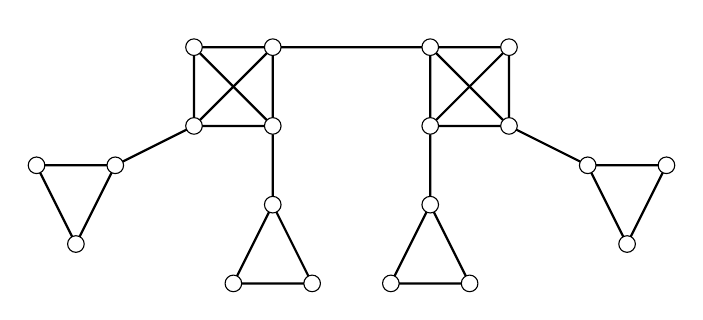
\begin{tikzpicture}[scale = 10]
\tikzstyle{VertexStyle} = []
\tikzstyle{EdgeStyle} = []
\tikzstyle{labeledStyle}=[shape = circle, minimum size = 6pt, inner sep = 1.2pt, draw]
\tikzstyle{unlabeledStyle}=[shape = circle, minimum size = 6pt, inner sep = 1.2pt, draw, fill]
\tikzstyle{Qstyle}=[shape = circle,minimum size = 6pt,inner sep = 1.2pt,draw]
\tikzstyle{NotQKkMinusOneStyle}=[shape = circle,minimum size = 6pt,inner sep = 1.2pt,draw]
\tikzstyle{endblockStyle}=[shape = circle,minimum size = 6pt,inner sep = 1.2pt,draw]
\Vertex[style = Qstyle, x = 0.450, y = 0.600, L = \tiny {}]{v0}
\Vertex[style = NotQKkMinusOneStyle, x = 0.550, y = 0.600, L = \tiny {}]{v1}
\Vertex[style = NotQKkMinusOneStyle, x = 0.450, y = 0.500, L = \tiny {}]{v2}
\Vertex[style = NotQKkMinusOneStyle, x = 0.550, y = 0.500, L = \tiny {}]{v3}
\Vertex[style = endblockStyle, x = 0.350, y = 0.450, L = \tiny {}]{v4}
\Vertex[style = endblockStyle, x = 0.300, y = 0.350, L = \tiny {}]{v5}
\Vertex[style = endblockStyle, x = 0.250, y = 0.450, L = \tiny {}]{v6}
\Vertex[style = endblockStyle, x = 0.600, y = 0.300, L = \tiny {}]{v7}
\Vertex[style = endblockStyle, x = 0.500, y = 0.300, L = \tiny {}]{v8}
\Vertex[style = endblockStyle, x = 0.550, y = 0.400, L = \tiny {}]{v9}
\Vertex[style = NotQKkMinusOneStyle, x = 0.750, y = 0.500, L = \tiny {}]{v10}
\Vertex[style = NotQKkMinusOneStyle, x = 0.850, y = 0.500, L = \tiny {}]{v11}
\Vertex[style = NotQKkMinusOneStyle, x = 0.750, y = 0.600, L = \tiny {}]{v12}
\Vertex[style = Qstyle, x = 0.850, y = 0.600, L = \tiny {}]{v13}
\Vertex[style = endblockStyle, x = 1.050, y = 0.450, L = \tiny {}]{v14}
\Vertex[style = endblockStyle, x = 1.000, y = 0.350, L = \tiny {}]{v15}
\Vertex[style = endblockStyle, x = 0.950, y = 0.450, L = \tiny {}]{v16}
\Vertex[style = endblockStyle, x = 0.800, y = 0.300, L = \tiny {}]{v17}
\Vertex[style = endblockStyle, x = 0.700, y = 0.300, L = \tiny {}]{v18}
\Vertex[style = endblockStyle, x = 0.750, y = 0.400, L = \tiny {}]{v19}
\Edge[label = \tiny {}, labelstyle={auto=right, fill=none}](v1)(v0)
\Edge[label = \tiny {}, labelstyle={auto=right, fill=none}](v1)(v2)
\Edge[label = \tiny {}, labelstyle={auto=right, fill=none}](v1)(v3)
\Edge[label = \tiny {}, labelstyle={auto=right, fill=none}](v2)(v0)
\Edge[label = \tiny {}, labelstyle={auto=right, fill=none}](v2)(v4)
\Edge[label = \tiny {}, labelstyle={auto=right, fill=none}](v3)(v0)
\Edge[label = \tiny {}, labelstyle={auto=right, fill=none}](v3)(v2)
\Edge[label = \tiny {}, labelstyle={auto=right, fill=none}](v4)(v5)
\Edge[label = \tiny {}, labelstyle={auto=right, fill=none}](v4)(v6)
\Edge[label = \tiny {}, labelstyle={auto=right, fill=none}](v5)(v6)
\Edge[label = \tiny {}, labelstyle={auto=right, fill=none}](v7)(v8)
\Edge[label = \tiny {}, labelstyle={auto=right, fill=none}](v7)(v9)
\Edge[label = \tiny {}, labelstyle={auto=right, fill=none}](v8)(v9)
\Edge[label = \tiny {}, labelstyle={auto=right, fill=none}](v9)(v3)
\Edge[label = \tiny {}, labelstyle={auto=right, fill=none}](v11)(v10)
\Edge[label = \tiny {}, labelstyle={auto=right, fill=none}](v11)(v12)
\Edge[label = \tiny {}, labelstyle={auto=right, fill=none}](v11)(v13)
\Edge[label = \tiny {}, labelstyle={auto=right, fill=none}](v12)(v1)
\Edge[label = \tiny {}, labelstyle={auto=right, fill=none}](v12)(v10)
\Edge[label = \tiny {}, labelstyle={auto=right, fill=none}](v13)(v10)
\Edge[label = \tiny {}, labelstyle={auto=right, fill=none}](v13)(v12)
\Edge[label = \tiny {}, labelstyle={auto=right, fill=none}](v14)(v15)
\Edge[label = \tiny {}, labelstyle={auto=right, fill=none}](v14)(v16)
\Edge[label = \tiny {}, labelstyle={auto=right, fill=none}](v15)(v16)
\Edge[label = \tiny {}, labelstyle={auto=right, fill=none}](v16)(v11)
\Edge[label = \tiny {}, labelstyle={auto=right, fill=none}](v17)(v18)
\Edge[label = \tiny {}, labelstyle={auto=right, fill=none}](v17)(v19)
\Edge[label = \tiny {}, labelstyle={auto=right, fill=none}](v18)(v19)
\Edge[label = \tiny {}, labelstyle={auto=right, fill=none}](v19)(v10)
\end{tikzpicture}
\caption{The construction when $k=5$ and $m=2$.}
\end{figure}

\begin{figure}
\centering
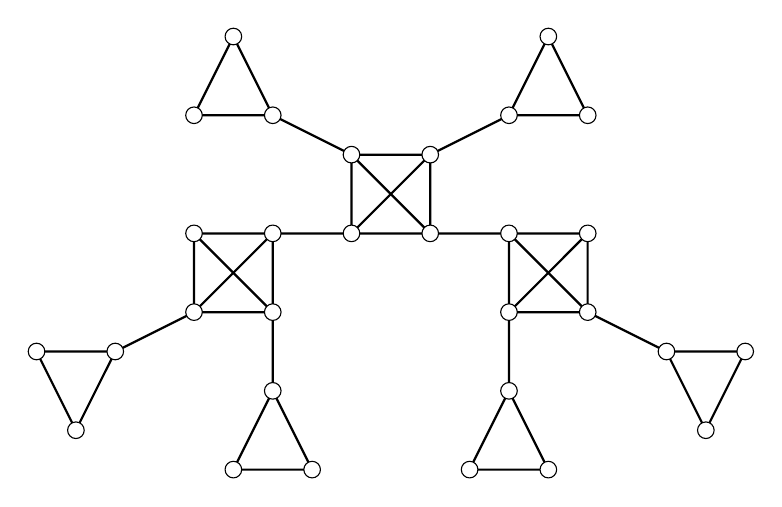
\begin{tikzpicture}[scale = 10]
\tikzstyle{VertexStyle} = []
\tikzstyle{EdgeStyle} = []
\tikzstyle{labeledStyle}=[shape = circle, minimum size = 6pt, inner sep = 1.2pt, draw]
\tikzstyle{unlabeledStyle}=[shape = circle, minimum size = 6pt, inner sep = 1.2pt, draw, fill]
\tikzstyle{NotQKkMinusOneStyle}=[shape = circle,minimum size = 6pt,inner sep = 1.2pt,draw]
\tikzstyle{Qstyle}=[shape = circle,minimum size = 6pt,inner sep = 1.2pt,draw]
\tikzstyle{endblockStyle}=[shape = circle,minimum size = 6pt,inner sep = 1.2pt,draw]
\Vertex[style = NotQKkMinusOneStyle, x = 0.650, y = 0.550, L = \tiny {}]{v0}
\Vertex[style = NotQKkMinusOneStyle, x = 0.750, y = 0.550, L = \tiny {}]{v1}
\Vertex[style = NotQKkMinusOneStyle, x = 0.650, y = 0.650, L = \tiny {}]{v2}
\Vertex[style = NotQKkMinusOneStyle, x = 0.750, y = 0.650, L = \tiny {}]{v3}
\Vertex[style = Qstyle, x = 0.450, y = 0.550, L = \tiny {}]{v4}
\Vertex[style = NotQKkMinusOneStyle, x = 0.550, y = 0.550, L = \tiny {}]{v5}
\Vertex[style = NotQKkMinusOneStyle, x = 0.450, y = 0.450, L = \tiny {}]{v6}
\Vertex[style = NotQKkMinusOneStyle, x = 0.550, y = 0.450, L = \tiny {}]{v7}
\Vertex[style = endblockStyle, x = 0.350, y = 0.400, L = \tiny {}]{v8}
\Vertex[style = endblockStyle, x = 0.300, y = 0.300, L = \tiny {}]{v9}
\Vertex[style = endblockStyle, x = 0.250, y = 0.400, L = \tiny {}]{v10}
\Vertex[style = endblockStyle, x = 0.600, y = 0.250, L = \tiny {}]{v11}
\Vertex[style = endblockStyle, x = 0.500, y = 0.250, L = \tiny {}]{v12}
\Vertex[style = endblockStyle, x = 0.550, y = 0.350, L = \tiny {}]{v13}
\Vertex[style = endblockStyle, x = 0.500, y = 0.800, L = \tiny {}]{v14}
\Vertex[style = endblockStyle, x = 0.450, y = 0.700, L = \tiny {}]{v15}
\Vertex[style = endblockStyle, x = 0.550, y = 0.700, L = \tiny {}]{v16}
\Vertex[style = NotQKkMinusOneStyle, x = 0.850, y = 0.450, L = \tiny {}]{v17}
\Vertex[style = NotQKkMinusOneStyle, x = 0.950, y = 0.450, L = \tiny {}]{v18}
\Vertex[style = NotQKkMinusOneStyle, x = 0.850, y = 0.550, L = \tiny {}]{v19}
\Vertex[style = Qstyle, x = 0.950, y = 0.550, L = \tiny {}]{v20}
\Vertex[style = endblockStyle, x = 1.150, y = 0.400, L = \tiny {}]{v21}
\Vertex[style = endblockStyle, x = 1.100, y = 0.300, L = \tiny {}]{v22}
\Vertex[style = endblockStyle, x = 1.050, y = 0.400, L = \tiny {}]{v23}
\Vertex[style = endblockStyle, x = 0.900, y = 0.250, L = \tiny {}]{v24}
\Vertex[style = endblockStyle, x = 0.800, y = 0.250, L = \tiny {}]{v25}
\Vertex[style = endblockStyle, x = 0.850, y = 0.350, L = \tiny {}]{v26}
\Vertex[style = endblockStyle, x = 0.900, y = 0.800, L = \tiny {}]{v27}
\Vertex[style = endblockStyle, x = 0.850, y = 0.700, L = \tiny {}]{v28}
\Vertex[style = endblockStyle, x = 0.950, y = 0.700, L = \tiny {}]{v29}
\Edge[label = \tiny {}, labelstyle={auto=right, fill=none}](v0)(v5)
\Edge[label = \tiny {}, labelstyle={auto=right, fill=none}](v1)(v0)
\Edge[label = \tiny {}, labelstyle={auto=right, fill=none}](v1)(v2)
\Edge[label = \tiny {}, labelstyle={auto=right, fill=none}](v1)(v3)
\Edge[label = \tiny {}, labelstyle={auto=right, fill=none}](v1)(v19)
\Edge[label = \tiny {}, labelstyle={auto=right, fill=none}](v2)(v0)
\Edge[label = \tiny {}, labelstyle={auto=right, fill=none}](v3)(v0)
\Edge[label = \tiny {}, labelstyle={auto=right, fill=none}](v3)(v2)
\Edge[label = \tiny {}, labelstyle={auto=right, fill=none}](v5)(v4)
\Edge[label = \tiny {}, labelstyle={auto=right, fill=none}](v5)(v6)
\Edge[label = \tiny {}, labelstyle={auto=right, fill=none}](v5)(v7)
\Edge[label = \tiny {}, labelstyle={auto=right, fill=none}](v6)(v4)
\Edge[label = \tiny {}, labelstyle={auto=right, fill=none}](v6)(v8)
\Edge[label = \tiny {}, labelstyle={auto=right, fill=none}](v7)(v4)
\Edge[label = \tiny {}, labelstyle={auto=right, fill=none}](v7)(v6)
\Edge[label = \tiny {}, labelstyle={auto=right, fill=none}](v8)(v9)
\Edge[label = \tiny {}, labelstyle={auto=right, fill=none}](v8)(v10)
\Edge[label = \tiny {}, labelstyle={auto=right, fill=none}](v9)(v10)
\Edge[label = \tiny {}, labelstyle={auto=right, fill=none}](v11)(v12)
\Edge[label = \tiny {}, labelstyle={auto=right, fill=none}](v11)(v13)
\Edge[label = \tiny {}, labelstyle={auto=right, fill=none}](v12)(v13)
\Edge[label = \tiny {}, labelstyle={auto=right, fill=none}](v13)(v7)
\Edge[label = \tiny {}, labelstyle={auto=right, fill=none}](v14)(v15)
\Edge[label = \tiny {}, labelstyle={auto=right, fill=none}](v14)(v16)
\Edge[label = \tiny {}, labelstyle={auto=right, fill=none}](v15)(v16)
\Edge[label = \tiny {}, labelstyle={auto=right, fill=none}](v16)(v2)
\Edge[label = \tiny {}, labelstyle={auto=right, fill=none}](v18)(v17)
\Edge[label = \tiny {}, labelstyle={auto=right, fill=none}](v18)(v19)
\Edge[label = \tiny {}, labelstyle={auto=right, fill=none}](v18)(v20)
\Edge[label = \tiny {}, labelstyle={auto=right, fill=none}](v19)(v17)
\Edge[label = \tiny {}, labelstyle={auto=right, fill=none}](v20)(v17)
\Edge[label = \tiny {}, labelstyle={auto=right, fill=none}](v20)(v19)
\Edge[label = \tiny {}, labelstyle={auto=right, fill=none}](v21)(v22)
\Edge[label = \tiny {}, labelstyle={auto=right, fill=none}](v21)(v23)
\Edge[label = \tiny {}, labelstyle={auto=right, fill=none}](v22)(v23)
\Edge[label = \tiny {}, labelstyle={auto=right, fill=none}](v24)(v25)
\Edge[label = \tiny {}, labelstyle={auto=right, fill=none}](v24)(v26)
\Edge[label = \tiny {}, labelstyle={auto=right, fill=none}](v25)(v26)
\Edge[label = \tiny {}, labelstyle={auto=right, fill=none}](v26)(v17)
\Edge[label = \tiny {}, labelstyle={auto=right, fill=none}](v23)(v18)
\Edge[label = \tiny {}, labelstyle={auto=right, fill=none}](v27)(v28)
\Edge[label = \tiny {}, labelstyle={auto=right, fill=none}](v27)(v29)
\Edge[label = \tiny {}, labelstyle={auto=right, fill=none}](v28)(v29)
\Edge[label = \tiny {}, labelstyle={auto=right, fill=none}](v28)(v3)
\end{tikzpicture}
\caption{The construction when $k=5$ and $m=3$.}
\end{figure}



\noindent
Note that $\frac{3k-5}{(k-5)(k-1)} < \frac{4(k-1)}{k^2 - 3k + 4}$ for $k \ge 7$.

In Section~\ref{discharging}, we will see that the bound we get on $d(G)$ is primarily a function of the $p(k)$ with which we 
apply Lemma~\ref{BoundFamilyWithKKMinusOne}: the smaller $p(k)$ is, the better bound we get on $d(G)$.  So it useful to note 
that the choice of $p(k)$ in Corollary~\ref{SmallP} is best possible.  We now give a construction to prove this.
Let $X$ be a $K_{k-1}$ with $k-3$ pendant edges.  At the end of each pendant edge, put a $K_{k-2}$.  Make a path of copies of $X$
by adding one edge between the $K_{k-1}$ in each copy of $X$ (in the only way possible to keep the degrees at most $k-1$).  Let 
$T$ be the path made like this from $m$ copies of $X$.  Now $q(T) = 2$ (from the end blocks), so if $T$ satisfies the bound in Lemma~\ref{BoundFamilyWithKKMinusOne}, then we must have
\begin{align*}
&m((k-1)(k-2) + (k-3)(k-2)(k-3) + 2(k-3)) + 2(m-1) \\
\le &(k-3 + p(k))(m)(k-1+(k-2)(k-3)) + f(k) + 2h(k),
\end{align*}
which reduces to
\[m(k-1) + 2m(k-3) + 2(m-1) \le (m)(k-1+(k-2)(k-3))p(k) + f(k) + 2h(k).\]
Now solving for $p(k)$ gives
\[p(k) \ge \frac{m(k-1)+2m(k-3)+2(m-1)-f(k)-2h(k)}{m((k-1)+(k-2)(k-3))},\] 
which simplifies to
\[p(k) \ge \frac{3k - 5}{k^2 - 4k + 5}-\frac{2+f(k)+2h(k)}{m(k^2-4k+5}.\]
Since we can make $m$ arbitrarily large, this implies $p(k)\ge \frac{3k-5}{k^2-4k+5}$, as desired.


\section{Discharging}\label{discharging}
%Lemma \ref{BasicGallaiTreeBound} is best possible as can be seen by the family of graphs with blocks on a path alternating %$K_{k-1}$ and $K_2$.  But we have reducible configurations (see the last section for the precise statements) that place %restrictions on $K_{k-1}$ blocks. To state these restrictions, we need the following auxiliary bipartite graph. 

\subsection{Overview and Discharging Rules}

Now we use the discharging method, together with the edge bound lemmas of the previous section, to give an improved bound on $d(G)$ 
for every $k$-critical graph $G$.  It is helpful to view our proof here as a refinement and strengthening of the proof in
Section~\ref{sec:gallai} of Gallai's bound.  For $T \in \T_k$, let $W^k(T)$ be the set of vertices of $T$ that are contained in 
some $K_{k-1}$ in $T$.  For a $k$-AT-critical graph $G$, let $\L(G)$ denote the subgraph of $G$ induced on the $(k-1)$-vertices and 
$\HH(G)$ the subgraph of $G$ induced on the $k$-vertices.     

Note that in the proof of Gallai's bound, all $(k+1)^+$-vertices finish with extra charge; $(k+1)$-vertices have extra
charge almost 1 and vertices of higher degree have even more.  Our idea to improve the bound on $d(G)$ is to have the 
$k$-vertices give slightly less charge, $\epsilon$, to their $(k-1)$-nbrs.  Now all $k^+$-vertices finish with extra charge.  
But components of $L(G)$ have less charge, so we need to give them more charge from $(k+1)^+$-neighbors.  
How much charge will each component $T$ of $L(G)$ receive? This depends on $||T||$.  If $||T||$ is small, then $T$ has many 
external neighbors, so $T$ will receive lots of charge.  If $||T||$ is large, then Lemma 3.2 implies that $q(T)$ is also large.  
So our plan is to send charge $\gamma$ to $T$ via each edge incident to a vertex in $W^k(T)$, i.e., one counted by 
$q(T)$.  (For comparison with Gallai's bound, we will have $\epsilon < \frac{k-3}{k^2-3} < \gamma$.)  If such an incident edge 
ends at a $(k+1)^+$-vertex $v$, then $v$ will still finish with sufficient charge.  Our concern, of course, is that a
$k$-vertex will give charge $\gamma$ to too many vertices in $W^k(T)$.  We would like to prove that each $k$-vertex has only a 
few neighbors in $W^k(T)$.  Unfortunately, we can not (and we believe this is false). However, we can prove that something similar 
is true.  We can assign each $k$-vertex to ``sponsor'' some adjacent vertices in $W^k(T)$, so that each $k$-vertex sponsors at 
most 3 such neighbors, and in each component $T$ of $L(G)$ at most two vertices in $W^k(T)$ go unsponsored.  This is an immediate
consequence of Lemma \ref{MultipleHighConfigurationEuler}, which says that the auxiliary bipartite graph $\B_k(G)$, defined in 
the next paragraph, is 2-degenerate.  And now, the details.

Let $\B_k(G)$ be the bipartite graph with one part $V(\HH(G))$ and the other part the components of $\L(G)$.  Put an edge 
between $y \in V(\HH(G))$ and a component $T$ of $\L(G)$ if and only if $N(y) \cap W^k(T) \ne \emptyset$.  Now 
Lemma~\ref{MultipleHighConfigurationEuler} says that $\B_k(G)$ is $2$-degenerate.
%
Let $\epsilon$ and $\gamma$ be parameters, to be chosen, such that $\epsilon < \gamma < 2\epsilon$. Our initial charge 
function is $\ch(v) = d_G(v)$.  We redistribute charge according to the following rules, applied successively.  
\begin{enumerate}
	\item Each $k^+$-vertex gives charge $\epsilon$ to each of its $(k-1)$-neighbors not in a $K_{k-1}$,
	\item Each $(k+1)^+$-vertex give charge $\gamma$ to each of its $(k-1)$-neighbors in a $K_{k-1}$,
	\item Let $Q = \B_k(G)$.  Repeat the following steps until $Q$ is empty.
	  \begin{enumerate}
	  	\item For each component $T$ of $\L(G)$ in $Q$ with degree at most two in $Q$ do the following:
	  	    \begin{enumerate}
	  	    	\item For each $v \in V(\HH(G)) \cap V(Q)$ such that $\card{N_G(v) \cap W^k(T)} = 2$, pick one $x \in N_G(v) \cap W^k(T)$ and send charge $\gamma$ from $v$ to $x$,
	  	    	\item Remove $T$ from $Q$.
	  	    \end{enumerate}
	  	\item For each vertex $v$ of $\HH(G)$ in $Q$ with degree at most two in $Q$ do the following:  
	  	    \begin{enumerate}
	  	        \item Send charge $\gamma$ from $v$ to each $x \in N_G(v) \cap W^k(T)$ for each component $T$ of $\L(G)$ where $vT \in E(Q)$.
	  	        \item Remove $v$ from $Q$.
	        \end{enumerate}
	  \end{enumerate}
	\item Have the vertices in each component of $\L(G)$ share their total charge equally.
\end{enumerate}

First, note that Step 3 will eventually result in Q being empty.  This is because $\B_k(G)$ is 2-degenerate, as shown in 
Lemma~\ref{MultipleHighConfigurationEuler}.  Next, consider a $k$-vertex $v$.  In (3bi) $v$ gives away $\gamma$ to each neighbor in 
at most two components of $\L(G)$.  So it is important that $v$ have few neighbors in these components.  Fortunately, this is true.
By Lemma~\ref{ConfigurationTypeOneEuler}, $v$ has at most 2 neighbors in any component of $\L(G)$.  Further, $v$ has at most one component where it has 2 neighbors.  Thus, in (3ai) and (3bi), $v$ gives away a total of at most $3\gamma$.  Finally, consider a component $T$.  In (3bi), $T$ receives charge $\gamma$ via every edge incident in $\B_k(G)$, except possibly two (that are still present when $v$ is deleted in (3aii)).  Again, by Lemma~\ref{MultipleHighConfigurationEuler}, no such $v$ has three neighbors in $T$.  Further, combining this with Steps (2) and (3ai), $T$ receives $\gamma$ along all but at most two incident edges leading to $k$-vertices.  Thus, $T$ receives charge at least $\gamma(q(T)-2)$ in Steps (2) and (3).

%Let $\ch^*(v)$ be the resulting charge function.  Here is some intuition for why this might be a useful refinement.  In (3b), $v$ sends charge to at most two different $T$ and so, by Lemma \ref{ConfigurationTypeOneEuler} (or our `beyond degree choosability' classification), $v$ loses charge at most $3\gamma$.  On the other hand, from (3a) each component $T$ of $\L(G)$ receives charge $\gamma$ for all but at most two non-separating vertices in a $K_{k-1}$ (the at most two is coming from Lemma \ref{ConfigurationTypeOneEuler} and the fact that we leave $T$ in $Q$ until it has degree at most two and when it does, we send up to two extra $\gamma$ to $T$ in (3ai) as needed). Note that (3ai) doesn't cause any $v \in V(\HH(G))$ to lose more than $3\gamma$, because it only gets enacted when the component $T$ is about to be removed, after that $v$ does not have two neighbors in another component. So, we can get each $T$ almost as much charge as we could hope for without losing too much from the $k$-vertices.  We don't have the same control over $(k+1)^+$-vertices, but it won't matter since they have extra charge to start with and sending $\gamma$ to every $(k-1)$-neighbor will leave enough charge (we'll use $\gamma < 2\epsilon$ here).

%To analyze this discharging procedure we need a bound like Lemma \ref{BasicGallaiTreeBound}, but taking into account the number of edges in $\B_k(G)$.  We can do this by taking into account the number of non-separating vertices in $K_{k-1}$'s in $T$.  To this end, for $T \in \T_k$, let $q(T)$ be the number of non-separating vertices in a $K_{k-1}$ in $T$.  We give a family of such bounds. 


\subsection{Analyzing the Discharging and the Main Result}
Finally, we analyze the charge received by each component $T$ of $\L(G)$.  We choose $\epsilon$ and $\gamma$ to maximize the minimum, over all vertices, of the final charge.  The following theorem is the main result of this paper.

\begin{thm}\label{UberTheorem}
	Let $k \ge 7$ and $\func{p}{\IN}{\IR}$, $\func{f}{\IN}{\IR}$, $\func{h}{\IN}{\IR}$.  If $G$ is a $k$-AT-critical graph, and $G\ne K_k$, then 
	\[d(G) \ge k-1 + \frac{2-p(k)}{k+2 + 3h(k) - p(k)},\]
	whenever $p$, $f$, and $k$ satisfy:
	\begin{enumerate}
	\item $f(k) \ge (k-1)(1- p(k) - h(k))$; and	
	    \item $p(k) \ge \frac{3}{k-2}$; and
		\item $p(k) \ge h(k) + 5 - k$; and
		\item $p(k) \ge \frac{2+h(k)}{k-2}$; and
		\item $(k-1)p(k) + (k-3)h(k) \ge k+1$; and
		\item $2(h(k) + 1) + f(k) \le 0$; and
		\item $p(k) + (k-5)h(k) \le k+1$.
	\end{enumerate}
\end{thm}

Before we prove Theorem~\ref{UberTheorem}, we show that two previous results on this problem follow immediately from this 
theorem.  
%In each case, we note that each $T\in \T_k$ with $K_{k-1} \not\subseteq T$ satisfies the hypothesis by
%Lemma~\eqref{BoundFamilyWithoutKKMinusOne} and each $T\in \T_k$ with $K_{k-1} \subseteq T$ satisfies the hypothesis by
%Lemma~\eqref{BoundFamilyWithKKMinusOne}.  
Note that (1)--(5) are the hypotheses of Lemma~\ref{BoundFamilyWithKKMinusOne}.
%
As a first test, let $p(k) = 1 - \frac{2}{k-1}$, $f(k) = -2$ and $h(k) = 0$.  Now the hypotheses of Theorem \ref{UberTheorem} are satisfied when $k\ge7$, and we get Gallai's bound: $d(G) \ge k-1 + \frac{k-3}{k^2-3}$. 
Next, let's use the Kostochka-Stiebitz bound, that is, $p(k) = \frac{4(k-1)}{k^2 - 3k + 4}$, $f(k) = -\frac{4(k^2-3k+2)}{k^2-3k+4}$ and $h(k) = \frac{k^2 - 3k}{k^2-3k+4}$.  Again, the hypotheses of Theorem \ref{UberTheorem} are satisfied when $k \ge 7$ and we get
\[d(G) \ge k-1 + \frac{2(k-2)(k-3)}{(k-1)(k^2 + 3k - 12)}.\]
This is exactly the bound in the paper of Kierstead and the second author~\cite{OreVizing}.  

Finally, to get our sharpest bound on $d(G)$, we use the bound in Corollary \ref{SmallP}, that is, $p(k) = \frac{3k-5}{k^2 - 4k + 5}$, $f(k) = -\frac{2(k-1)(2k-5)}{k^2 - 4k + 5}$, and $h(k) = \frac{k(k-3)}{k^2 - 4k + 5}$.  The hypotheses of Theorem \ref{UberTheorem} are satisfied when $k\ge7$ and we get $d(G) \ge k-1 + \frac{(k-3)(2k-5)}{k^3 + k^2 - 15k + 15}.$
 This is better than the bound in~\cite{OreVizing} for $k \ge 7$.  We record this as our main corollary.

\begin{cor}\label{MainCor}
If $G$ is a $k$-AT-critical graph, with $k\ge 7$, and $G\ne K_k$, then
 \[d(G) \ge k-1 + \frac{(k-3)(2k-5)}{k^3 + k^2 - 15k + 15}.\]
\end{cor}

Now we prove Theorem~\ref{UberTheorem}
\begin{proof}[Proof of Theorem~\ref{UberTheorem}]
Our discharging procedure in the previous section gives charge $\epsilon$ to a component $T$ for every incident edge not ending in a $K_{k-1}$.  The number of such edges is exactly
\[-q(T) + \sum_{v \in V(T)} (k-1 - d_T(v)) = (k-1)\card{T} - 2\size{T} - q(T),\]
so let $A(T)$ denote this quantity.  When $K_{k-1} \subseteq T$, since (1)--(5) hold, Lemma~\ref{BoundFamilyWithKKMinusOne} implies that
\[2\size{T} \le (k-3 + p(k))\card{T} + f(k) + h(k)q(T).\]
So, when $K_{k-1} \subseteq T$ we get
\begin{align*}
    A(T) & \ge (k-1)\card{T} - q(T) - ((k-3 + p(k))\card{T} + f(k) + h(k)q(T))\\
         &  =(2-p(k))\card{T} - f(k) - (h(k) + 1)q(T).
\end{align*}
Hence, in total $T$ receives charge at least
\begin{align*}
    \epsilon A(T) + \gamma(q(T) - 2) &\ge \epsilon(2-p(k))|T| - \epsilon f(k) - \epsilon (h(k)+1)q(T) +\gamma q(T)-2\gamma \\
    & = \epsilon(2-p(k))|T| + q(T)(\gamma - \epsilon (h(k)+1)) - (2\gamma + \epsilon f(k))
\end{align*}
Our goal is to make $\epsilon(2-p(k))$ as large as possible, while ensuring that the final two terms are nonnegative.  To make the second term 0, we let $\gamma = \epsilon(h(k) + 1)$.  Now the final term becomes $-\epsilon(2(h(k)+1)+f(k))$.
%
%That happens because $T$ receives charge on all but at most two of its non-separating vertices in a $K_{k-1}$; that is, in %discharging steps 2 and 3, $T$ receives charge at least $\gamma\max\set{0, q(G) - 2}$.    = \epsilon\parens{2-p(k)}\card{T} - %\epsilon \parens{f(k) + 2(h(k) + 1)}.\]
%
For simplicity, we have added, as (6), that $2(h(k) + 1) + f(k) \le 0$.  (Since we typically take $h(k) > 0$, as in Corollary~\ref{MainCor}, it is precisely this requirement that necessitates the use of $f(k)$ in Lemma~\ref{BoundFamilyWithKKMinusOne}.)  Thus, $T$ receives charge at least
\[\epsilon\parens{2-p(k)}\card{T},\]
so each of its vertices gets at least $\epsilon(2-p(k))$.
We also need each $k$-vertex to end with enough charge, and each of these loses at most $3\gamma+(k-3)\epsilon$.  So we take
\[1 - (3\gamma + (k-3)\epsilon) = \epsilon\parens{2-p(k)},\]
which gives
\[\epsilon = \frac{1}{k+2 + 3h(k) - p(k)},\]
\[\gamma = \frac{h(k)+1}{k+2 + 3h(k) - p(k)}.\]
Thus, after discharging, each $k$-vertex finishes with charge at least $k-1+\epsilon(2-p(k))$.  The same bound holds for each $(k-1)$-vertex in a component $T$ with a $K_{k-1}$.

When $K_{k-1} \not \subseteq T$, we have $q(T) = 0$.  Applying Lemma \ref{BoundFamilyWithoutKKMinusOne} with $f(k) = 0$ and $p(k)$ as in the present, we get 
\[2\size{T} \le (k-3 + p(k))\card{T},\]
and hence
\[A(T) \ge (2-p(k))\card{T},\]
which is sufficient charge.

It remains to check that the $(k+1)^+$-vertices don't give away too much charge.  Let $v$ be a $(k+1)^+$-vertex. Now $v$ ends with charge at least
\[d(v) - \gamma d(v) = (1-\gamma)d(v) \ge (1-\gamma)(k+1) = (k+1)\frac{k+1 + 2h(k) - p(k)}{k+2 + 3h(k) - p(k)},\]
so we need that the inequality
\[(k+1)\frac{k+1 + 2h(k) - p(k)}{k+2 + 3h(k) - p(k)} \ge k-1 + \frac{2-p(k)}{k+2 + 3h(k) - p(k)}\]
holds.  This inequality reduces to
\[p(k) + (k-5)h(k) \le k+1.\]
For simplicity, we have added this as (7), since it is easily satisfied by the $p$, $f$, and $h$ we want to use.
\end{proof}

The reason that we require $k\ge 7$ in Theorem~\ref{UberTheorem} (and Corollary~\ref{MainCor}) is that the proof uses Lemma~\ref{MultipleHighConfigurationEuler}.
However, for $k\in\{5,6\}$, Lemma~\ref{MultipleHighConfigurationEulerLopsided} can play an analogous role.  
For $k\ge 7$, Lemma~\ref{MultipleHighConfigurationEuler} implies that if $G$ has no reducible configuration, then $B_k(G)$ is
2-degenerate.  For $k\in\{5,6\}$, Lemma~\ref{MultipleHighConfigurationEulerLopsided} implies that we can reduce $\B_k(G)$ to 
the empty graph by repeatedly deleting either a tree component vertex $v$ with $d_{\B_k(G)}(v)\le 1$ or else a vertex $w$ in 
$V(\B_k(G))\cap V(\HH(G))$ with $d_{\B_k(G)}(v)\le 3$.  Thus, in the discharging, the tree corresponding to $v$ receives charge 
at least $\gamma(q(T)-1)$ on edges ending at vertices in $W^k(T)$.  Similarly, each $k$-vertex gives away charge at most 
$4\gamma+(k-4)\epsilon$.  Now, to find the optimal value of $\epsilon$, as in the proof of Theorem~\ref{UberTheorem}, we 
solve $(1-(4\gamma+\epsilon(k-4))=(2-p(k))\epsilon$.  This gives $\epsilon = \frac1{k+2+4h(k)-p(k)}$ and, again, 
$\gamma=\epsilon(h(k)+1)$.  In place of hypothesis (6), we have the slightly weaker requirement $h(k)+1+f(k)\le 0$.  The result is 
the following theorem and corollary, for $k\in\{5,6\}$.

\begin{thm}\label{Uber56}
	Let $k \in\{5,6\}$ and $\func{p}{\IN}{\IR}$, $\func{f}{\IN}{\IR}$, $\func{h}{\IN}{\IR}$.  If $G$ is a $k$-AT-critical graph, and $G\ne K_k$, then 
	\[d(G) \ge k-1 + \frac{2-p(k)}{k+2 + 4h(k) - p(k)},\]
	whenever $p$, $f$, and $k$ satisfy:
	\begin{enumerate}
	\item $f(k) \ge (k-1)(1- p(k) - h(k))$; and	
	    \item $p(k) \ge \frac{3}{k-2}$; and
		\item $p(k) \ge h(k) + 5 - k$; and
		\item $p(k) \ge \frac{2+h(k)}{k-2}$; and
		\item $(k-1)p(k) + (k-3)h(k) \ge k+1$; and
		\item $h(k) + 1 + f(k) \le 0$; and
		\item $p(k) + (k-5)h(k) \le k+1$.
	\end{enumerate}
\end{thm}

To get the best bound on $d(G)$, as in Theorem~\ref{UberTheorem}, we use $p(k) = \frac{3k-5}{k^2 - 4k + 5}$, $f(k) = -\frac{2(k-1)(2k-5)}{k^2 - 4k + 5}$, and $h(k) = \frac{k(k-3)}{k^2 - 4k + 5}$.
\begin{cor}\label{MinorCor}
If $G$ is a $k$-AT-critical graph, with $k\in\{5,6\}$, and $G\ne K_k$, then
 \[d(G) \ge k-1 + \frac{(k-3)(2k-5)}{k^3 + 2k^2 - 18k + 15}.\]
\end{cor}

Possible improvements:

\begin{enumerate}
	\item Use a better bound on average degree of Gallai trees.  i would like to find the best possible family in the form here.  How does this bound compare to the hand waiving one in the other document?
	\item In the discharging, the $k$-vertices lost $3\gamma$ even though they had degree two in $Q$ because of the possibility of two edges into one component.  Can we get this to $2\gamma$ somehow, like maybe we can order our picking so that no vertex is picked before the component where it has two edges has been removed.   
	\item Related to the previous item, improved reducible configurations, a less restrictive condition in Lemma \ref{MultipleHighConfigurationEuler} taking into account the two edges to a component issue.
\end{enumerate}

\section{Reducible Configurations}
\begin{defn}
	A graph $G$ is \emph{AT-reducible} to $H$ if $H$ is a nonempty induced subgraph of $G$ which is $f_H$-AT where $f_H(v) \DefinedAs \delta(G) + d_H(v) - d_G(v)$ for all $v \in V(H)$.  
	If $G$ is not AT-reducible to any nonempty induced subgraph, then it is \emph{AT-irreducible}.
\end{defn}

This first lemma tells us how a single high vertex can interact with the low vertex subgraph.  This is the version Hal and i used, it (and more) follows from the classification in ``mostlow''.

\begin{lem}\label{ConfigurationTypeOneEuler}
Let $k \ge 5$ and let $G$ be a graph with $x \in V(G)$ such that:
\begin{enumerate}
\item $K_k \not \subseteq G$; and
\item $G-x$ has $t$ components $H_1, H_2, \ldots, H_t$, and all are in $\T_k$; and
\item $d_G(v) \leq k - 1$ for all $v \in V(G-x)$; and
\item $\card{N(x) \cap W^k(H_i)} \ge 1$ for $i \in \irange{t}$; and
\item $d_G(x) \ge t+2$.
\end{enumerate}

\noindent Then $G$ is $f$-AT where $f(x) = d_G(x) - 1$ and $f(v) = d_G(v)$ for all $v \in V(G - x)$.
\end{lem}

To deal with more than one high vertex we need the following auxiliary bipartite graph.  For a graph $G$, $\set{X, Y}$ a partition of $V(G)$ and $k \ge 4$, let $\B_k(X, Y)$ be the bipartite graph with one part $Y$ and the other part the components of $G[X]$.  Put an edge between $y \in Y$ and a component $T$ of $G[X]$ if and only if $N(y) \cap W^k(T) \ne \emptyset$.   The next lemma tells us that we have a reducible configuration if this bipartite graph has minimum degree at least three.  

\begin{lem}
	\label{MultipleHighConfigurationEuler} Let $k\ge7$ and let $G$ be a graph with
	$Y\subseteq V(G)$ such that: 
	\begin{enumerate}
		\item $K_{k}\not\subseteq G$; and 
		\item the components of $G-Y$ are in $\T_{k}$; and 
		\item $d_{G}(v)\leq k-1$ for all $v\in V(G-Y)$; and 
		\item with $\B\DefinedAs\B_{k}(V(G-Y),Y)$ we have $\delta(\B)\ge3$. 
	\end{enumerate}
	\noindent Then $G$ has an induced subgraph $G'$ that is $f$-AT where $f(y)=d_{G'}(y)-1$
	for $y\in Y$ and $f(v)=d_{G'}(v)$ for all $v\in V(G'-Y)$.\end{lem}

We also have the following version with asymmetric degree condition on $\B$.  The point here is that this works for $k \ge 5$.  As we'll see in the next section, the consequence is that we trade a bit in our size bound for the proof to go through with $k \in \set{5,6}$.

\begin{lem}
	\label{MultipleHighConfigurationEulerLopsided} Let $k \ge 5$ and let $G$ be a graph with
	$Y\subseteq V(G)$ such that: 
	\begin{enumerate}
		\item $K_{k}\not\subseteq G$; and 
		\item the components of $G-Y$ are in $\T_{k}$; and 
		\item $d_{G}(v)\leq k-1$ for all $v\in V(G-Y)$; and 
		\item with $\B \DefinedAs \B_k(V(G-Y), Y)$ we have $d_{\B}(y) \ge 4$ for all $y \in Y$ and $d_{\B}(T) \ge 2$ for all components $T$ of $G-Y$.
	\end{enumerate}
	\noindent Then $G$ has an induced subgraph $G'$ that is $f$-AT where $f(y)=d_{G'}(y)-1$
	for $y\in Y$ and $f(v)=d_{G'}(v)$ for all $v\in V(G'-Y)$.\end{lem}



\bibliographystyle{amsplain}
\bibliography{GraphColoring1}
\end{document}

 
